\documentclass[aspectratio=169]{beamer}
\usetheme[style=noir]{fhtw}
\usepackage{preamble}

\title[Rapid Prototyping]{Rapid Prototyping}
\subtitle{CI - ASSIST HEIDI}
\author{Alija Sabic, \glsentrytext{msc}}
\mail{sabic@technikum-wien.at}
\institute{Department Electronic Engineering}

\begin{document}

\begin{frame}[plain]
    \titlepage
    \nocite{aigner:rapid-prototyping}
    \nocite{fasterman:2012}
    \nocite{benchoff:2014:1}
    \nocite{benchoff:2014:2}
    \nocite{hubs}
\end{frame}

\section{Literature}

\begin{frame}
    \begin{itemize}
        \item Slides are based on Benjamin Aigner, \acs{msc}: \res{aigner:rapid-prototyping}
        \item \res{fasterman:2012}
        \item \res{benchoff:2014:1}
        \item \res{benchoff:2014:2}
        \item \res{hubs}
    \end{itemize}
\end{frame}

\section{Rapid Prototyping}

\begin{frame}
    \begin{definition}
        An embedded system is a computer system --- a combination of computer processor, computer memory, and input/output peripheral devices --- that has a dedicated function within a larger mechanical or electronic system (Source: \href{https://en.wikipedia.org/wiki/Embedded_system}{Wikipedia - Embedded Systems}).
    \end{definition}
    \vspace{-1em}
    \begin{figure}
        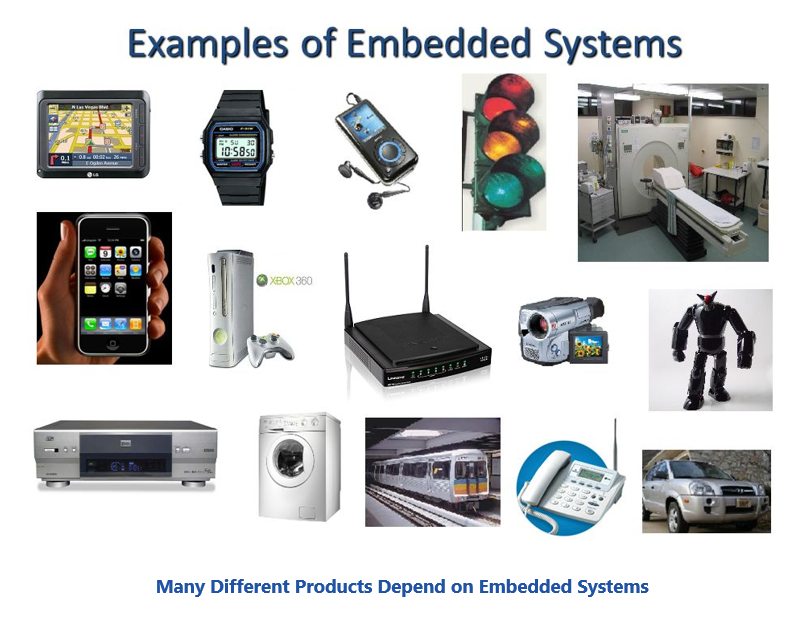
\includegraphics[width=0.5\textwidth]{microcontroller/embedded-system-examples.png}
        \caption{\glsentrydesc{es} examples.}
    \end{figure}
\end{frame}
\subsection{Technologies}
\begin{frame}
    \begin{figure}
        \includegraphics<1>[width=0.95\linewidth]{rapid-prototyping/additive-manufacturing-poster-3d_hubs.pdf}
        % \includegraphics<2>[width=0.3\linewidth,trim=8mm 6cm 34cm 75mm, clip]{rapid-prototyping/additive-manufacturing-poster-3d_hubs.pdf}
        % \includegraphics<3>[width=0.3\linewidth,trim=7cm 3cm 30cm 75mm, clip]{rapid-prototyping/additive-manufacturing-poster-3d_hubs.pdf}
        \caption{Additive manufacturing technologies}
    \end{figure}
\end{frame}
\subsection{\glsentrydesc{fdm}}
\begin{frame}
    \begin{figure}
        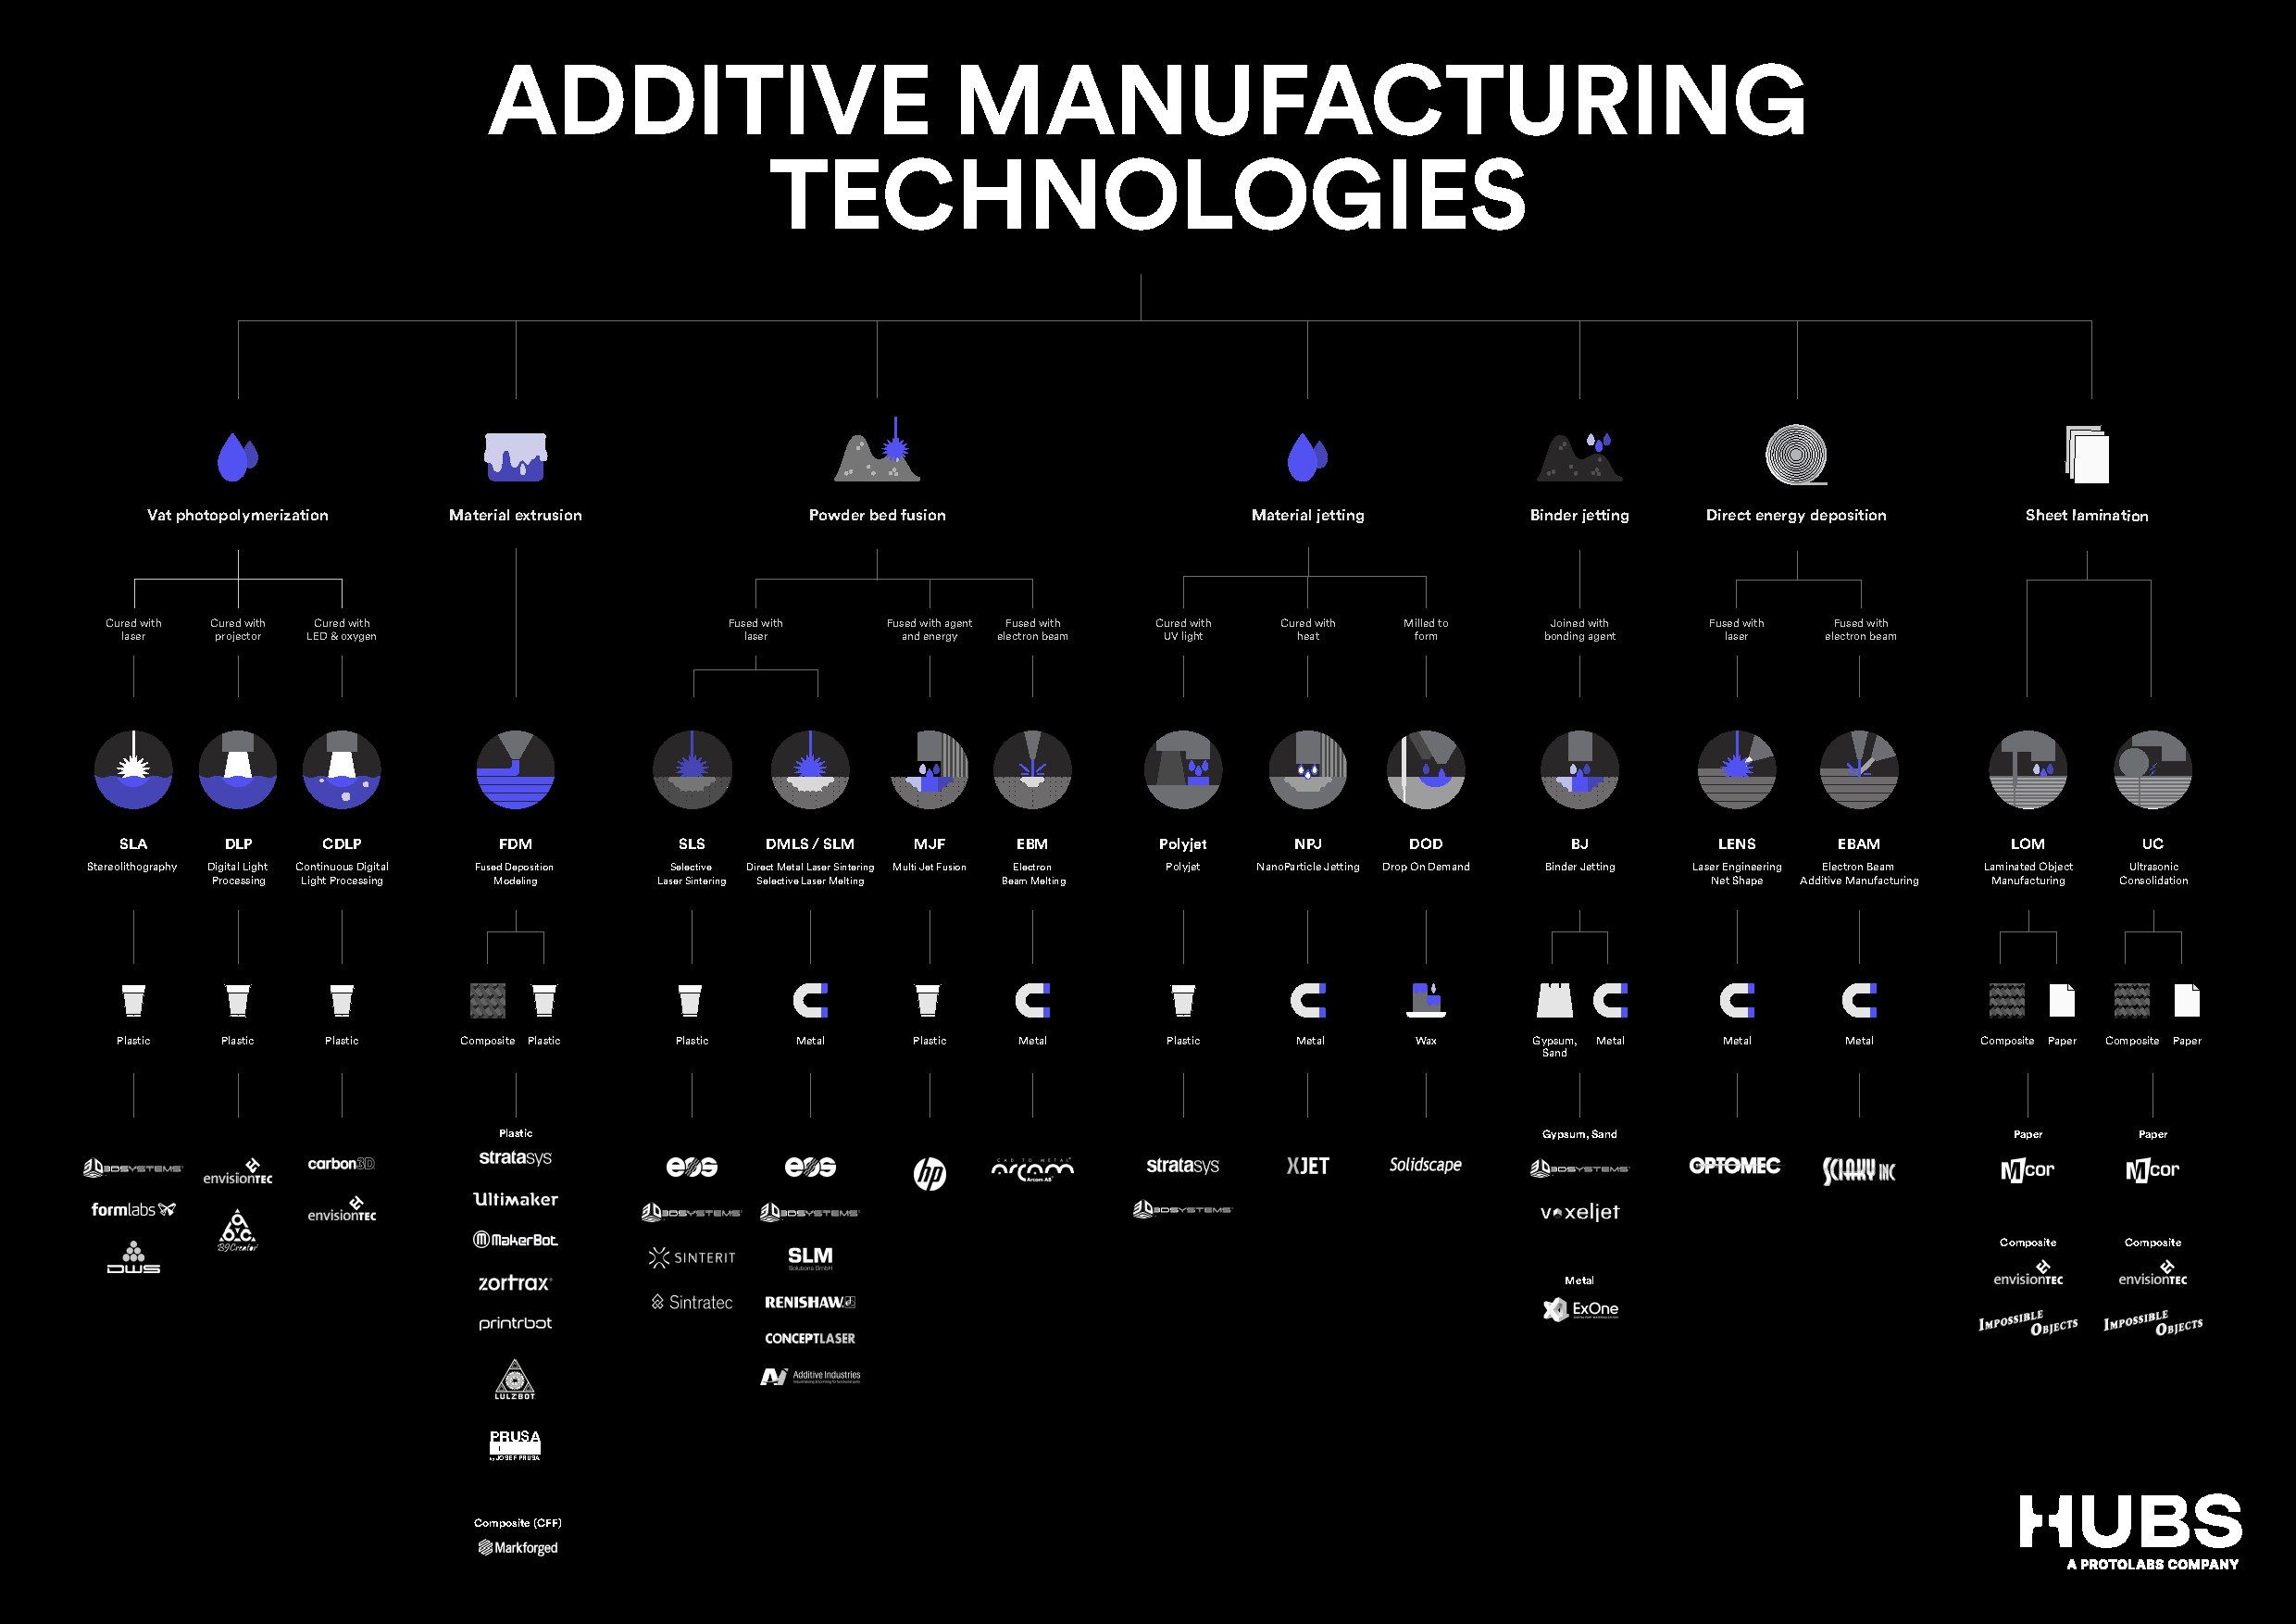
\includegraphics[width=0.3\linewidth,trim=75mm 17.5cm 30.5cm 5cm, clip]{rapid-prototyping/additive-manufacturing-poster-3d_hubs.pdf}
        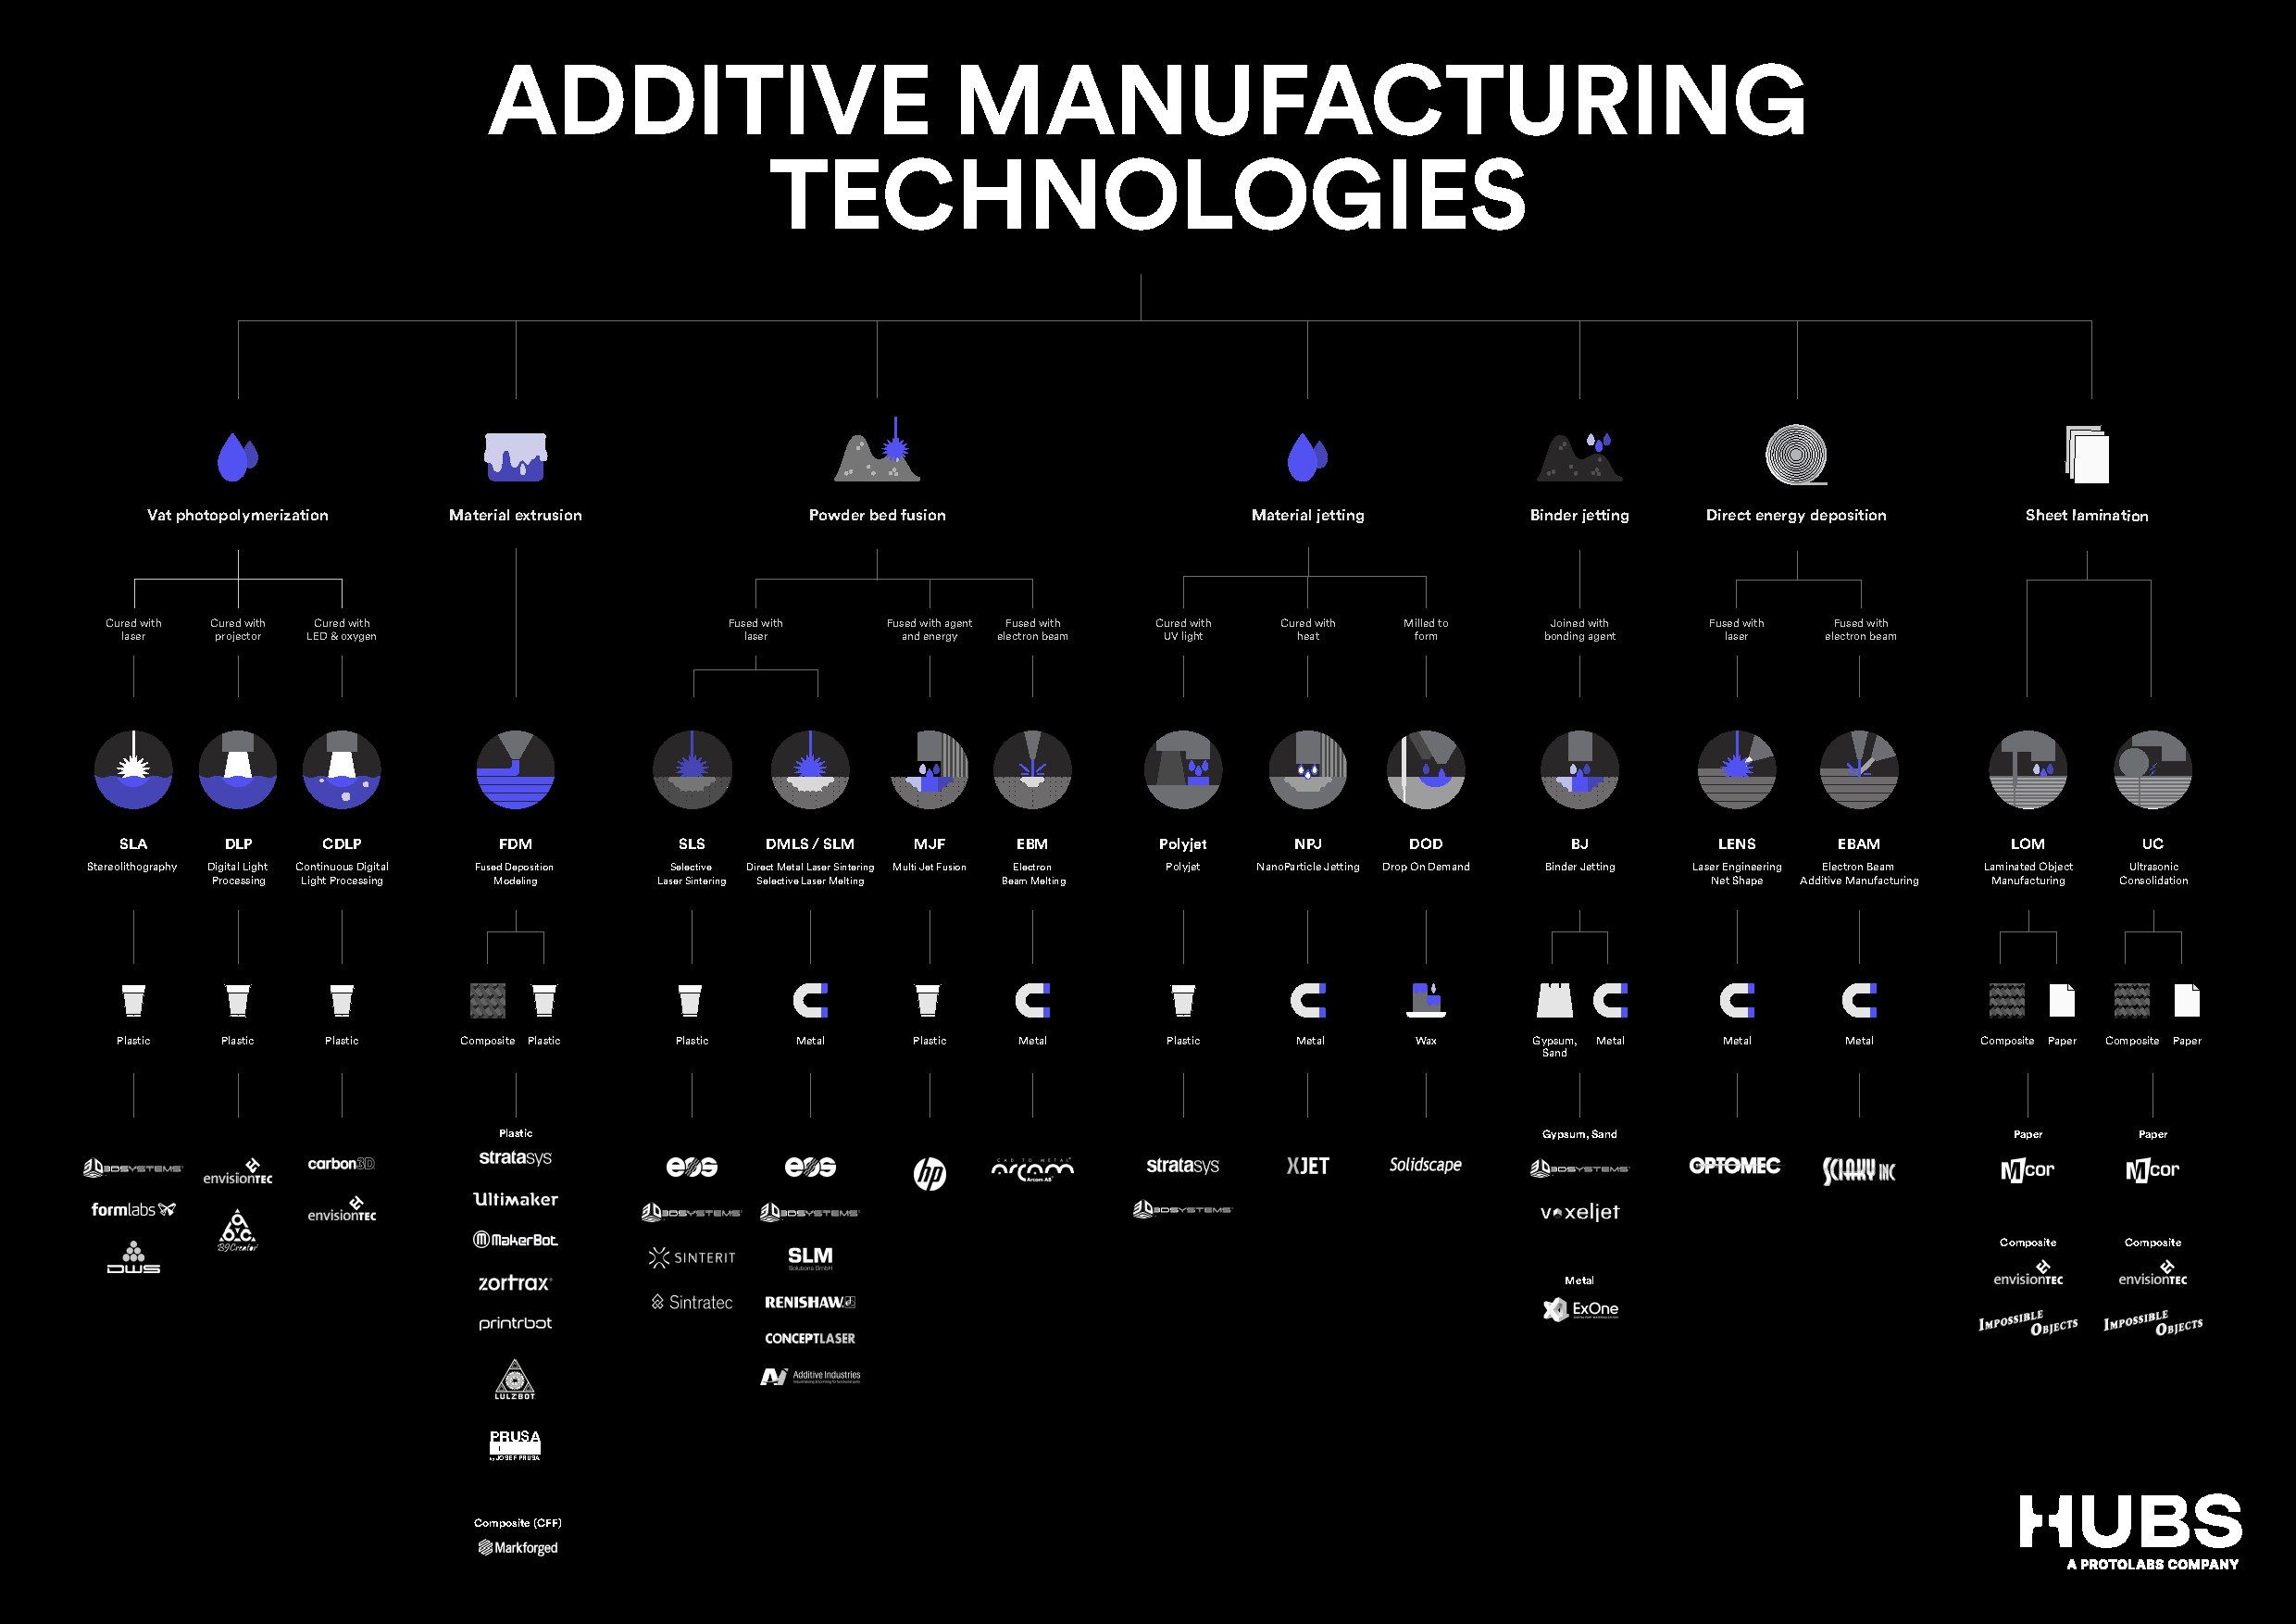
\includegraphics[width=0.3\linewidth,trim=75mm 10.5cm 30.5cm 12cm, clip]{rapid-prototyping/additive-manufacturing-poster-3d_hubs.pdf}
        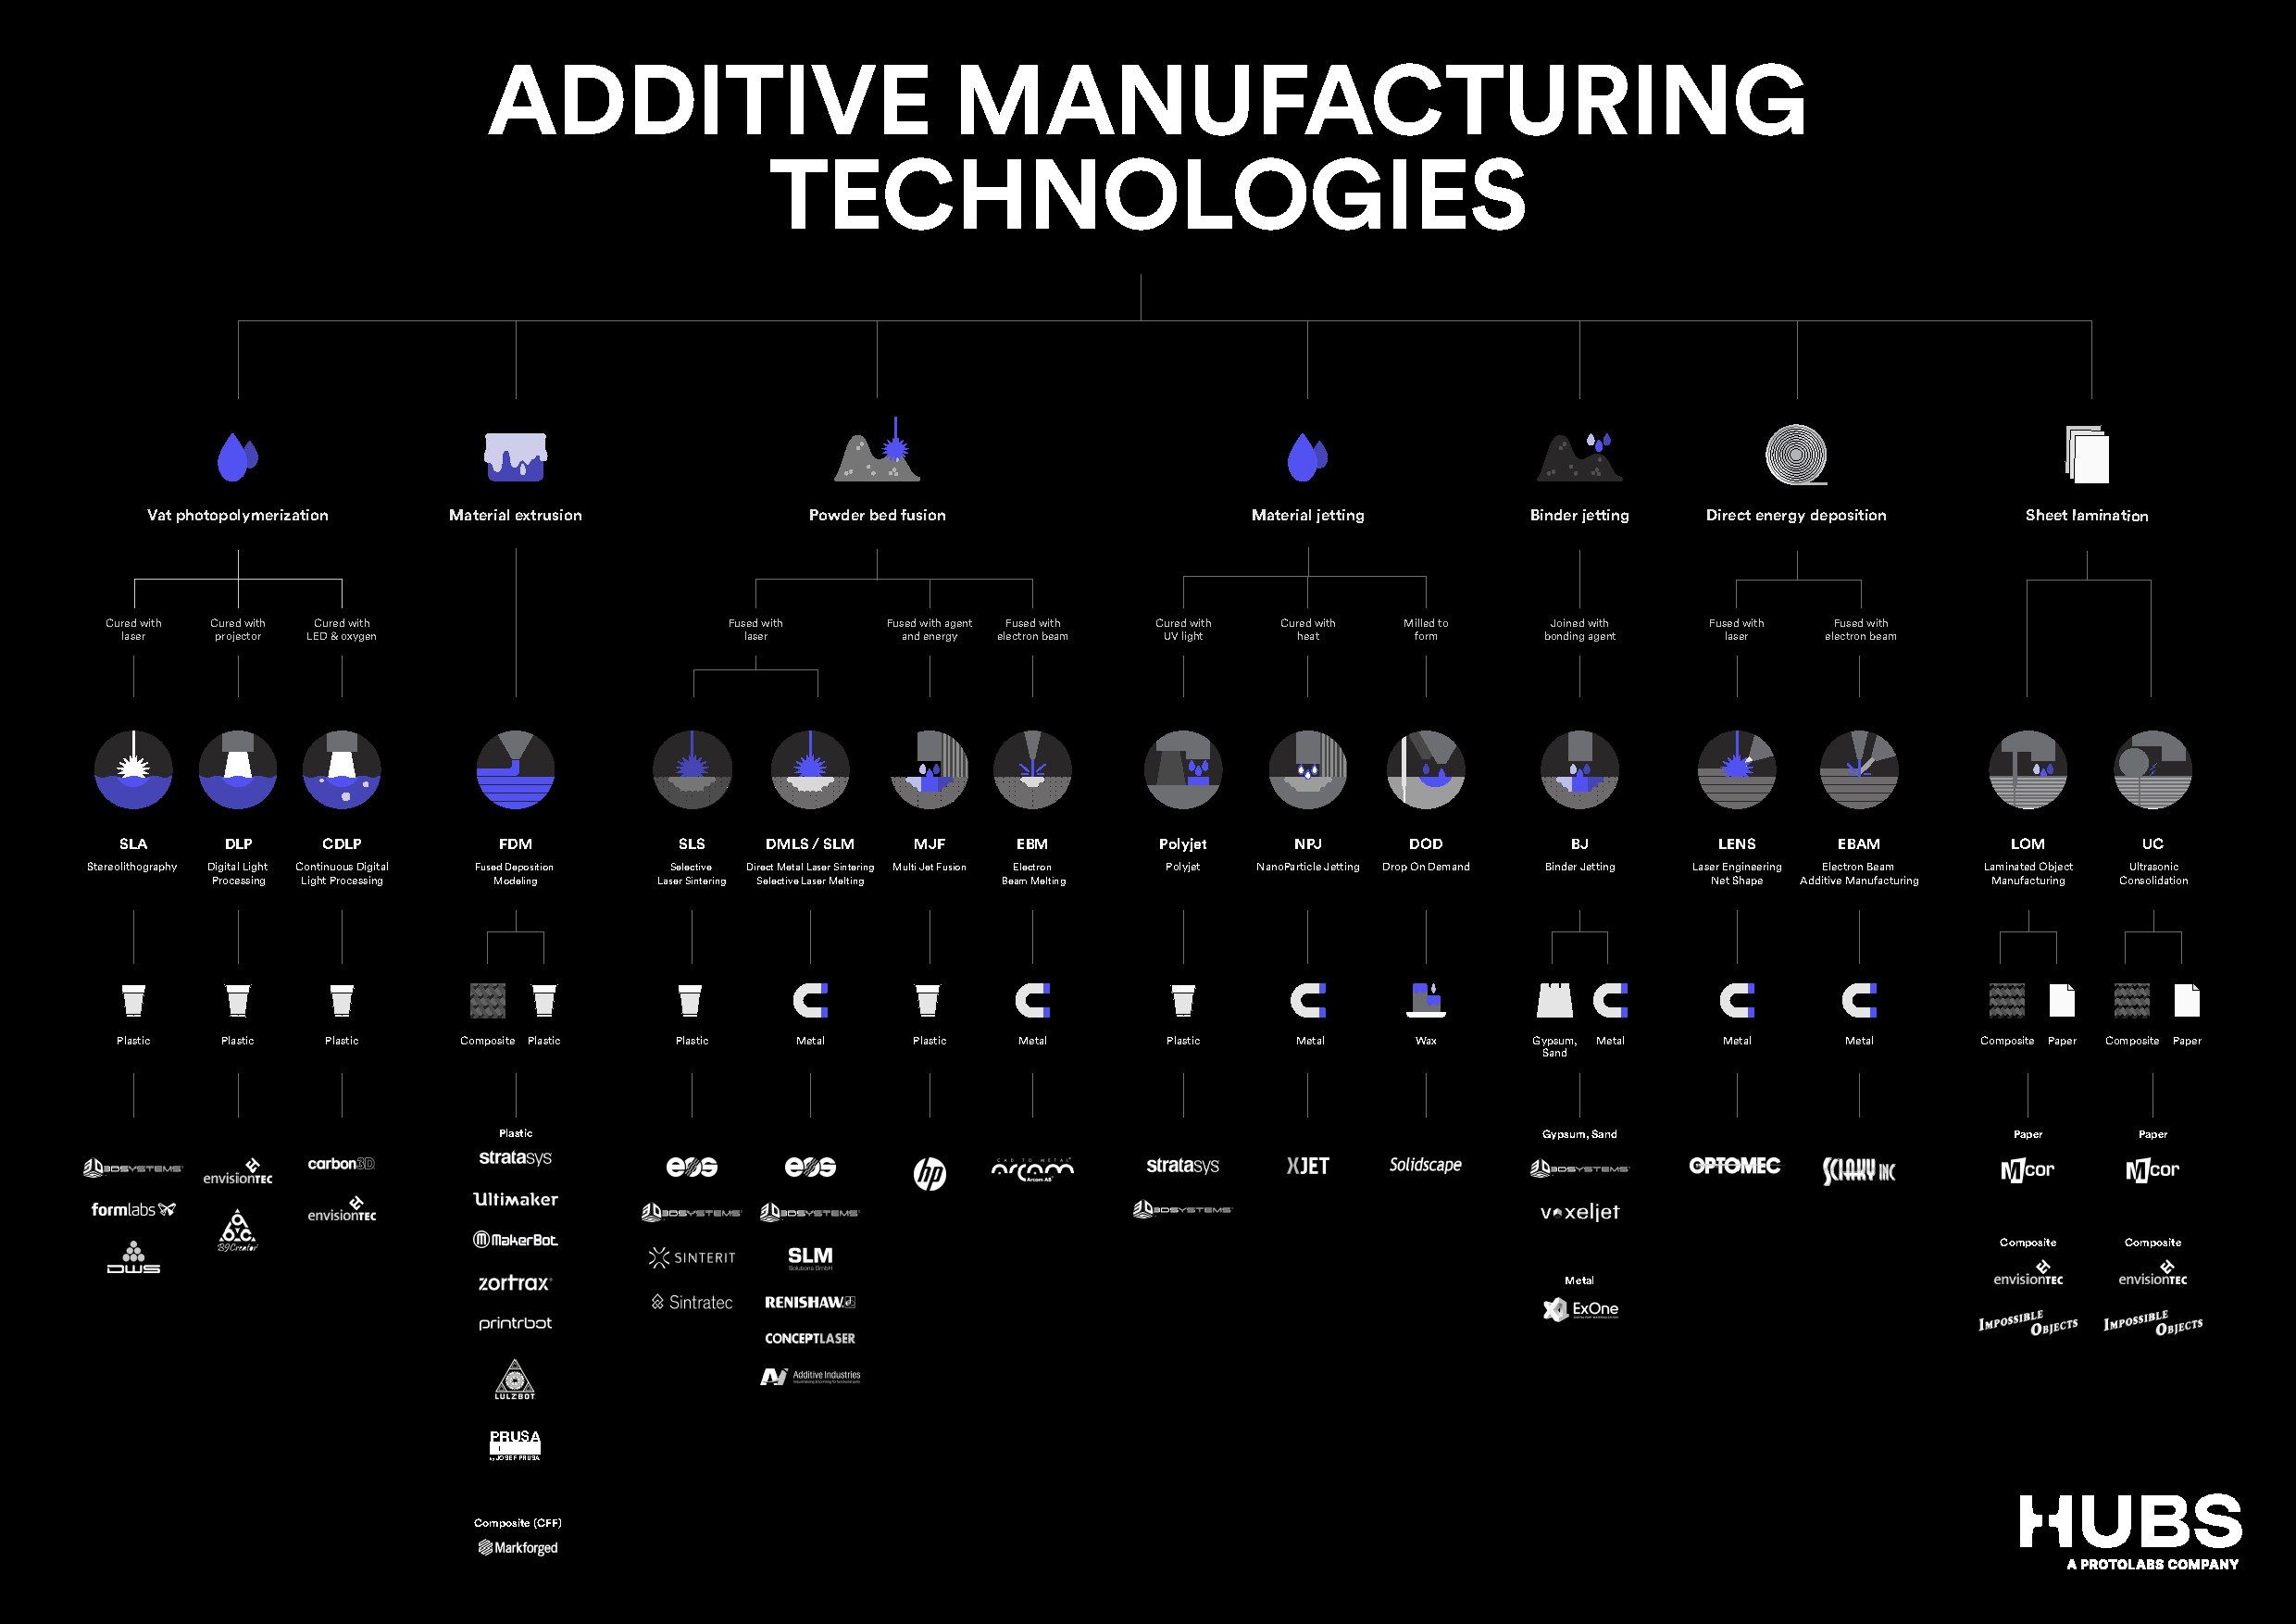
\includegraphics[width=0.3\linewidth,trim=75mm 2.5cm 30.5cm 20cm, clip]{rapid-prototyping/additive-manufacturing-poster-3d_hubs.pdf}
        \caption{\glsentrydesc{fdm}}
    \end{figure}
    \begin{itemize}
        \item \gls{fdm} \texttrademark
        \item \gls{fff} (free term)
    \end{itemize}
\end{frame}
\subsection{FabLabs}
\begin{frame}
    % \par Fabrication Laboratory
    \begin{itemize}
        \item Open workplaces
        \item Typical machines
              \begin{itemize}
                  \item 3D printers
                  \item Laser cutters
                  \item \acs{cnc} machines
                  \item Presses
                  \item \ldots
              \end{itemize}
        \item Vienna: HappyLab or MetaLab
    \end{itemize}
    \begin{columns}
        \begin{column}{0.55\textwidth}
            \begin{figure}
                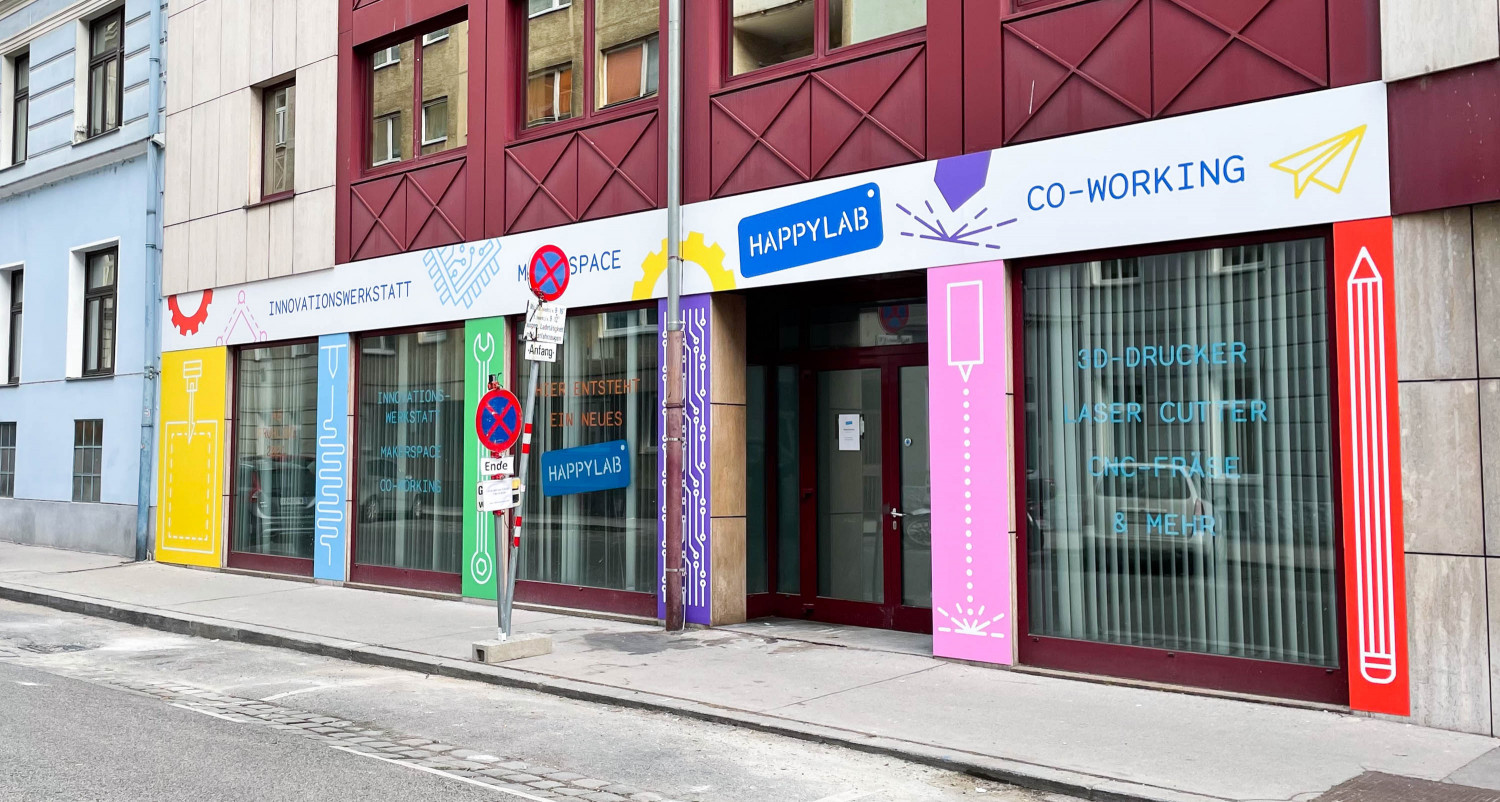
\includegraphics[height=30mm]{rapid-prototyping/happylab.jpg}
                \caption{HappyLab}
            \end{figure}
        \end{column}
        \begin{column}{0.45\textwidth}
            \begin{figure}
                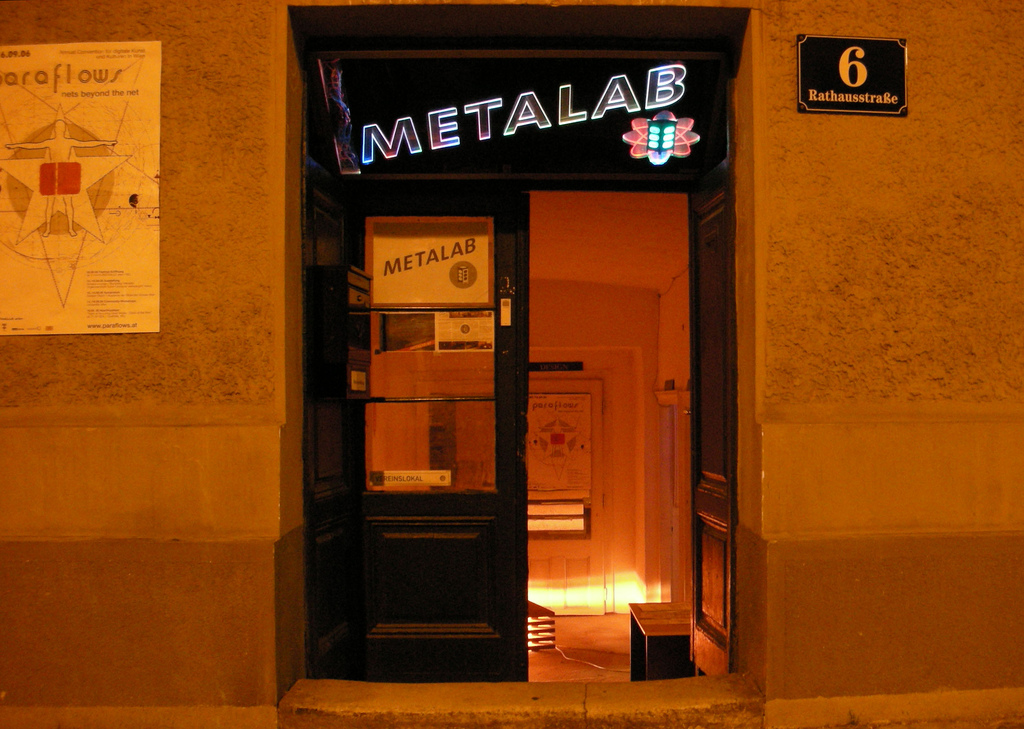
\includegraphics[height=30mm]{rapid-prototyping/metalab.jpg}
                \caption{MetaLab}
            \end{figure}
        \end{column}
    \end{columns}
\end{frame}
\subsection{Social Impact}
\begin{frame}
    \begin{block}{The Economist, A third industrial revolution}
        ``As manufacturing goes digital, a third great change is now gathering space.
        It will allow things to be made economically in much smaller numbers, more flexibly and with a much lower input of labor.''
    \end{block}
    \begin{itemize}
        \item Decentralization of production (shift towards consumers)
        \item Sustainability and democratization $\rightarrow$ maker movement
        \item Discussion about patents and licensing
    \end{itemize}
\end{frame}

\section{3D Printing}

\subsection{\glsentrydesc{fdm}}
\begin{frame}
    \begin{itemize}
        \item Material (filament) is applied layer by layer
        \item Movable print head
        \item Precision down to \SI{0.1}{\milli\meter} possible (typical: \SIrange{0.3}{0.5}{\milli\meter})
        \item Speed and precision depends on diameter (typical \SI{0.4}{\milli\meter})
        \item Material: \SI{1.75}{\milli\meter} or \SI{3}{\milli\meter} diameter
    \end{itemize}
\end{frame}

\begin{frame}
    \begin{figure}
        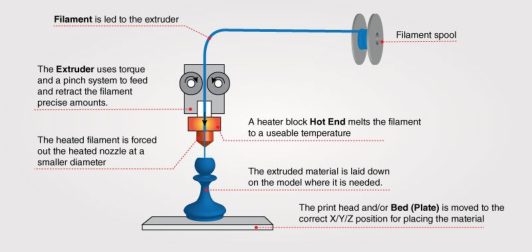
\includegraphics[width=\textwidth]{rapid-prototyping/fused-deposition-modeling.pdf}
        \caption{\glsentrydesc{fdm}}
    \end{figure}
\end{frame}

\subsection{\glsentrydesc{dlp}}
\begin{frame}
    \begin{itemize}
        \item Liquid photopolymers (photosensitive)
        \item Printed object is pulled out of the material from bottom to top
        \item Each layer is partially cured by \acs{uv} light projector
        \item Higher precision than with \acs{fff} is possible
        \item Prices are also decreasing (inexpensive printers $\approx$ \SI{250}{\sieuro})
    \end{itemize}
\end{frame}

\begin{frame}
    \begin{figure}
        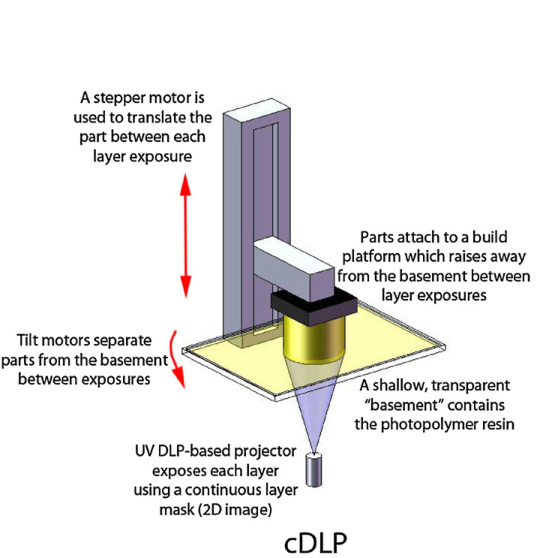
\includegraphics[height=7cm]{rapid-prototyping/digital-light-processing.pdf}
        \caption{\glsentrydesc{dlp}}
    \end{figure}
\end{frame}
\subsection{\glsentrydesc{sls}}
\begin{frame}
    \begin{itemize}
        \item Laser beam heats powdery material
        \item Melting or sintering
        \item Expensive to purchase
        \item High powder wear
    \end{itemize}
    \begin{figure}
        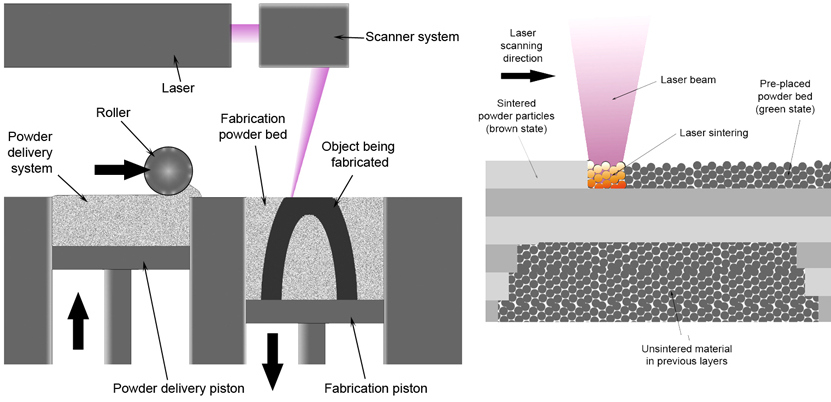
\includegraphics[height=5cm]{rapid-prototyping/selective-laser-sintering.jpg}
        \caption{\glsentrydesc{sls}}
    \end{figure}
\end{frame}
\subsection{Materials}
\begin{frame}
    \begin{itemize}
        \item \acs{pla}
              \begin{itemize}
                  \item Polyactide, biocompatible/biodegradable
                  \item Printing temperature: $\approx$ \SI{200}{\celsius}
                  \item Easiest material for \acs{fff} printing
              \end{itemize}
        \item Biocompounds
              \begin{itemize}
                  \item Plastics produced from biological feedstock
                  \item Various properties, e.g. GreenTec from Extrudr
                        \begin{itemize}
                            \item Biodegradable
                            \item Food safe
                            \item Dimensionally stable up to \SI{120}{\celsius}
                        \end{itemize}
              \end{itemize}
    \end{itemize}
\end{frame}

\begin{frame}
    \begin{itemize}
        \item \acs{abs}
              \begin{itemize}
                  \item \acl{abs} copolymers
                  \item Recyclable (non-biodegradable)
                  \item Printing temperature: $\approx$ \SI{220}{\celsius}
                  \item Somewhat difficult material for \acs{fff} printing
                  \item Very resilient
              \end{itemize}
        \item \acs{petg}
              \begin{itemize}
                  \item \acl{petg}
                  \item Recyclable (non-biodegradable)
                  \item Printing temperature: $\approx$ \SI{250}{\celsius}
                  \item Food safe
                  \item Easy to use
                  \item Not all printers can work without problems at this high temperature
              \end{itemize}
    \end{itemize}
\end{frame}

\begin{frame}
    \begin{itemize}
        \item \acs{pva}
              \begin{itemize}
                  \item \acl{pva}
                  \item Water-soluble
                  \item Printing temperature: $\approx$ \SI{200}{\celsius}
                  \item Used as support material and dissolved in water after printing
              \end{itemize}
        \item Photopolymer
              \begin{itemize}
                  \item Used in \acs{dlp} printers
                  \item Composition depends on manufacturer
              \end{itemize}
    \end{itemize}
\end{frame}
\subsection{Workflow}
\begin{frame}
    \begin{enumerate}
        \item Plan/model the model (or use existing model)
        \item Export the model in \acs{stl} format (\acs{cad} software)
        \item Convert \acs{stl} file into printer compatible layer model (slicer)
        \item Export layer model to G-code (for \acs{fff}, but not for \acs{dlp})
        \item Print
    \end{enumerate}
\end{frame}
\subsection{\glsentrytext{stl} Files}
\begin{frame}
    \begin{itemize}
        \item \acl{stl}
        \item Description by single triangle facets
        \item Generates only an approximation
        \item Especially difficult: curves/round bodies
    \end{itemize}
    \begin{exampleblock}{}
        Generated from 3D modeling software or downloaded from the internet.
        Platform compatible, can be used for any generative manufacturing process.
    \end{exampleblock}
\end{frame}
\subsection{Slicing}
\begin{frame}
    \begin{itemize}
        \item Creates a layer model from \acs{stl} files
        \item Every movement of the print head is calculated (only for \acs{fff})
        \item Many adjustment possibilities
        \item Accuracy/speed/material of print if defined here
    \end{itemize}
    \begin{exampleblock}{}
        The slicer generates G-code from the \acs{stl} file.
        This G-code depends on: printer, material, speed, accuracy, etc.
        In \acs{dlp} printing, a projected image is created for each layer.
    \end{exampleblock}
\end{frame}
\subsection{G-code}
\begin{frame}
    \begin{itemize}
        \item \acs{rs}-274, originally for \acs{cnc} machines (only for \acs{fff})
        \item Pure text description of the execution of the commands
        \item G-code is sent to the 3D printer either via an external medium (\acs{usb} stick, \acs{sd} card) or via cable
        \item \texttt{G} \ldots\, movement of the tool/print head
        \item \texttt{M} \ldots\, miscellaneous functions
        \item \texttt{F} \ldots\, feed
        \item \texttt{X/Y/Z} \ldots\, absolute or relative x, y, z coordinates
    \end{itemize}
    \begin{exampleblock}{}
        G-code expresses the exact instructions for the 3D printer.
        The commands are printer and material specific.
    \end{exampleblock}
\end{frame}

\begin{frame}
    \begin{listing}[H]
        \inputsource[]{gcode}{gcode/example.gcode}
        \caption{G-code example}
        \label{lst:gcode:example}
    \end{listing}
\end{frame}
\subsection{Software and Platforms}
\subsubsection{Thingiverse}
\begin{frame}
    \begin{itemize}
        \item Platform for the exchange of 3D models
        \item Extensive collection
        \item Many \acs{at} models
        \item Attention: not all models are suitable for \acs{fff}
    \end{itemize}
    \begin{figure}
        % https://www.thingiverse.com/thing:1104936
        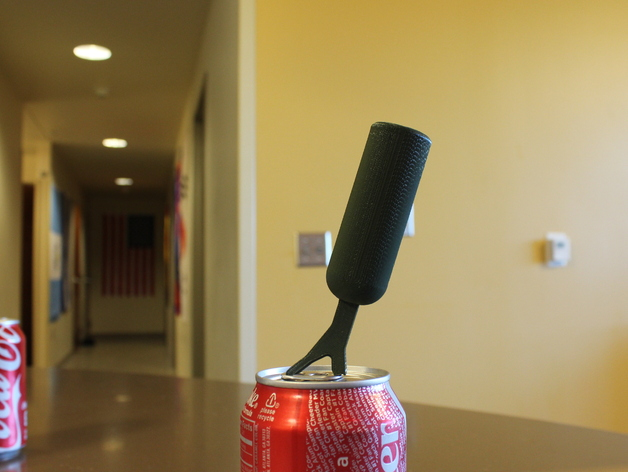
\includegraphics[height=4cm]{rapid-prototyping/thingiverse-canopener.jpg}
        \caption{Pop Can Opener: Designed for People with Prosthetics or Severe Arthritis}
    \end{figure}
\end{frame}
\subsubsection{\glsentrytext{cad}}
\begin{frame}
    \begin{columns}
        \hspace{0.1\textwidth}
        \begin{column}[t]{0.4\textwidth}
            \begin{itemize}
                \item Commercial
                      \begin{itemize}
                          \item SolidWorks
                          \item Auto\acs{cad}
                          \item \acs{catia}
                          \item SketchUp
                          \item Inventor
                          \item Fusion360
                          \item SolidEdge
                      \end{itemize}
            \end{itemize}
            % \end{frame}
        \end{column}
        \begin{column}[t]{0.4\textwidth}
            % \subsubsection{\glsentrytext{cad} - Free}
            % \begin{frame}
            \begin{itemize}
                \item Free
                      \begin{itemize}
                          \item Free\acs{cad}
                          \item Blender
                          \item \textcolor{tw-gray}{AutoDesk Inventor}
                          \item \textcolor{tw-gray}{OnShape}
                          \item OpenSCAD
                          \item Libre\acs{cad}
                          \item 123D (discontinued)
                      \end{itemize}
            \end{itemize}
        \end{column}
        \hspace{0.1\textwidth}
    \end{columns}
\end{frame}

\section{Laser Cutter}

\subsection{Technology}
\begin{frame}
    \begin{itemize}
        \item Compact development board based on the RP2040 microcontroller
        \item Dual-core \acs{arm} Cortex-M0+ processor with a clock speed of \SI{133}{\mega\hertz}
        \item \SI{2}{\mebi\byte} of onboard flash memory
        \item Integrated \acs{wifi} and \ac{ble} connectivity
        \item 6-axis \ac{imu} for motion sensing
        \item Built-in microphone for audio input
        \item U-blox NINA-W102 module for wireless connectivity
    \end{itemize}
    \begin{figure}
        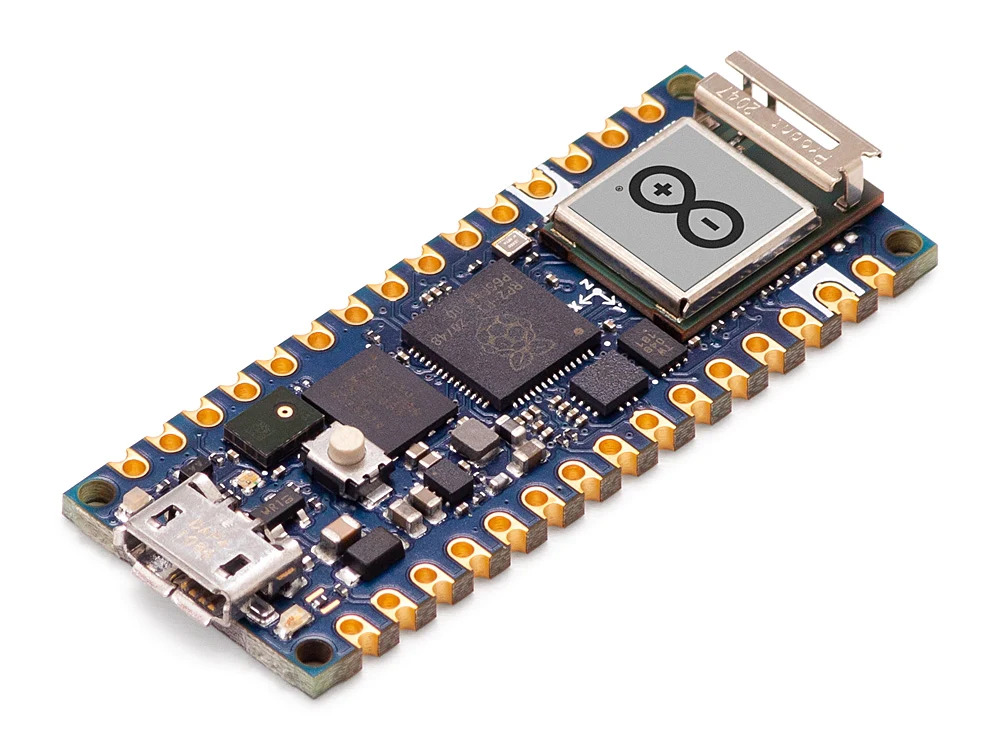
\includegraphics[height=2cm]{microcontroller/arduino/rp2040/rp2040-connect-isometric.jpg}
        \caption{Arduino\textregistered{} Nano RP2040 Connect: Board}
    \end{figure}
\end{frame}
\subsection{Laser}
\begin{frame}
    \begin{itemize}
        \item Electromagnetic waves
        \item High intensity
        \item Monochromatic wavelength
        \item Sharp focussing
        \item For laser cutting: infrared light
    \end{itemize}
\end{frame}
\subsection{Advantages}
\begin{frame}
    \begin{itemize}
        \item Complex outlines possible
        \item Precise
        \item Fast
        \item Low minimum number of copies
        \item Cutting/engraving in one step possible
    \end{itemize}
\end{frame}
\subsection{Disadvantages}
\begin{frame}
    \begin{itemize}
        \item High acquisition cost
        \item Hazard protection
        \item Low electrical efficiency ($\approx$ \SI{20}{\percent})
        \item Repeatability (especially for low cost machines)
        \item Many, but not all materials possible
    \end{itemize}
\end{frame}
\subsection{Products}
\begin{frame}
    \begin{columns}
        \begin{column}[t]{0.5\textwidth}
            \begin{itemize}
                \item Manufacturer
                      \begin{itemize}
                          \item Trotec
                          \item Epilog
                                %   \item GCC
                          \item Thunderlaser
                          \item \ldots
                      \end{itemize}
            \end{itemize}
        \end{column}
        \begin{column}[t]{0.5\textwidth}
            \begin{itemize}
                \item \SIrange{20}{400}{\watt}
                \item Industrial grade: up to \SI{8}{\kilo\watt}
            \end{itemize}
        \end{column}
    \end{columns}
    % \begin{itemize}
    %     \item Manufacturer
    %             \begin{itemize}
    %                 \item Trotec
    %                 \item Epilog
    %                 \item GCC
    %                 \item Thunderlaser
    %                 \item \ldots
    %             \end{itemize}
    %     \item \SIrange{20}{400}{\watt}
    %     \item Industrial grade: up to \SI{8}{\kilo\watt}
    % \end{itemize}
    \begin{columns}
        \begin{column}{0.5\textwidth}
            \begin{figure}
                % https://www.happylab.at/de_vie/ausstattung#lasercutter
                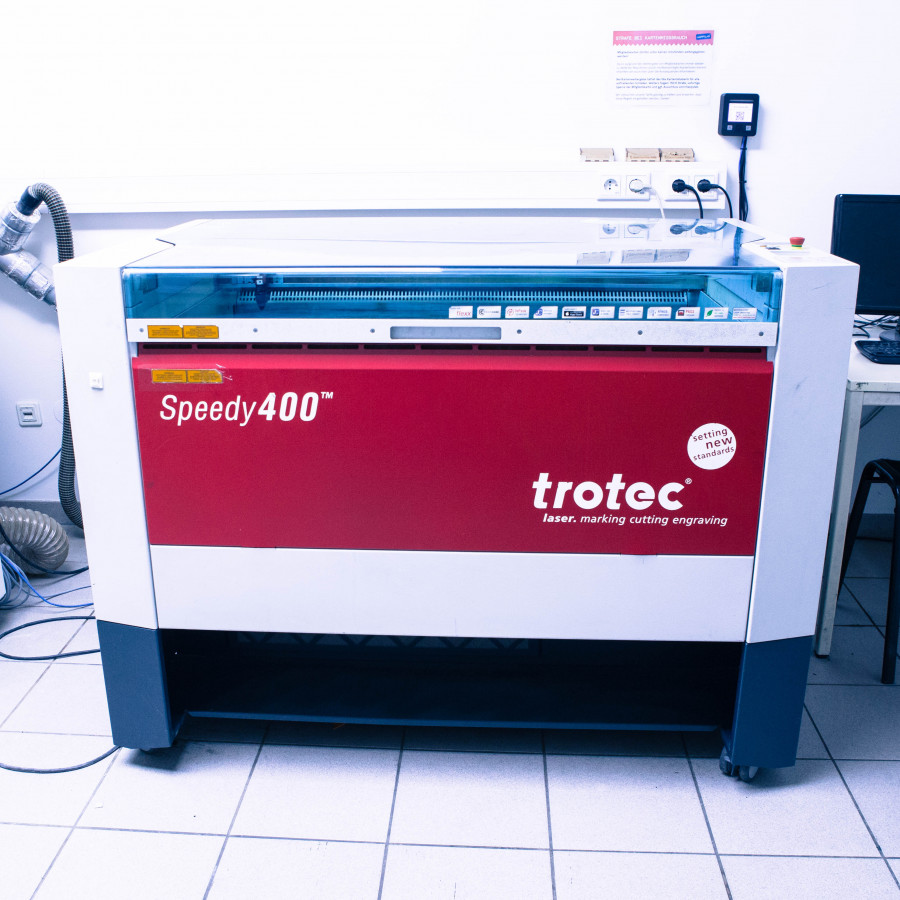
\includegraphics[height=4cm, trim=0mm 1.5cm 0mm 1cm, clip]{rapid-prototyping/trotec-speedy-400.jpg}
                \caption{Trotec: Speedy 400}
            \end{figure}
        \end{column}
        \begin{column}{0.5\textwidth}
            \begin{figure}
                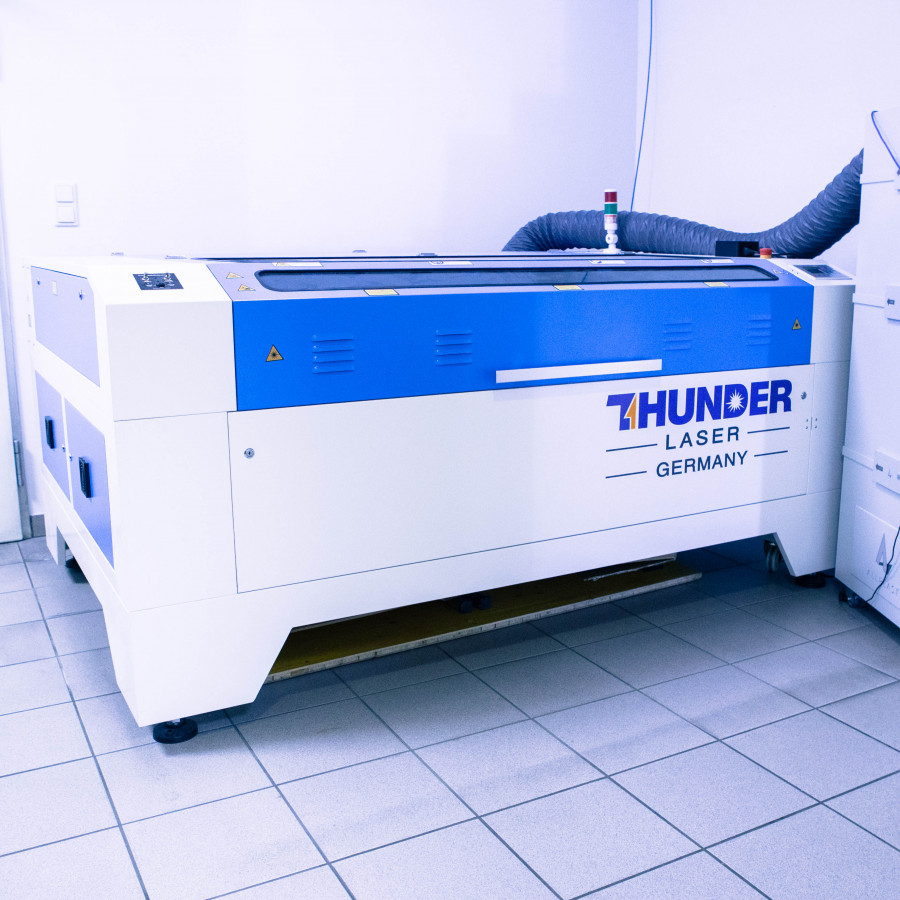
\includegraphics[height=4cm, trim=0mm 1.5cm 0mm 1cm, clip]{rapid-prototyping/thunderlaser-nova63.jpg}
                \caption{Thunderlaser: Nova63}
            \end{figure}
        \end{column}
    \end{columns}
\end{frame}

% \begin{frame}
% \end{frame}
\subsection{Examples}
\begin{frame}
    \begin{figure}
        % https://www.hackschool.org/post/creating-tabbed-boxes-in-inkscape
        \includegraphics<1>[width=0.9\textwidth]{rapid-prototyping/laser-cut-box.jpg}
        \includegraphics<2>[height=7.5cm, angle=90, origin=c]{rapid-prototyping/laser-cut-inkscape.png}
        \caption{Laser Cut: Box of Wood}
    \end{figure}
\end{frame}

\begin{frame}
    \begin{figure}
        % https://makerdesignlab.com/tutorials-tips/laser-cutting-beginners-guide/
        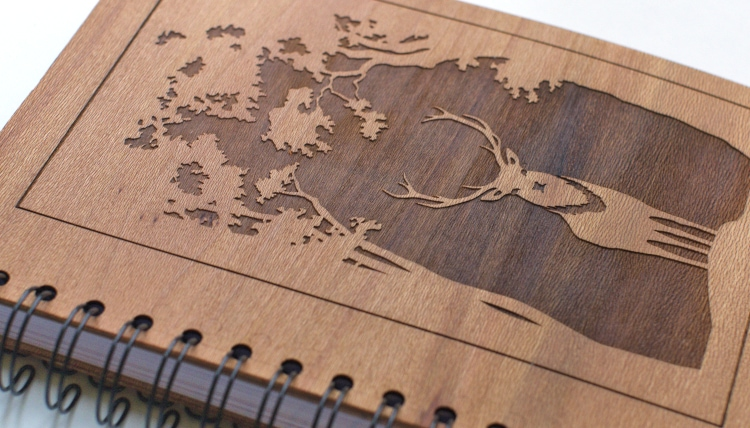
\includegraphics[width=\textwidth]{rapid-prototyping/laser-cut-engraving.jpg}
        \caption{Laser Cut: Engraving}
    \end{figure}
\end{frame}


\section{Other Technologies}

\subsection{Lego \texttrademark}
\begin{frame}
    \begin{itemize}
        \item Very fast
        \item Modular
        \item Many different elements
        \item Combination with other technologies
    \end{itemize}
    \begin{figure}
        % https://www.instructables.com/LEGO-3d-Printer/
        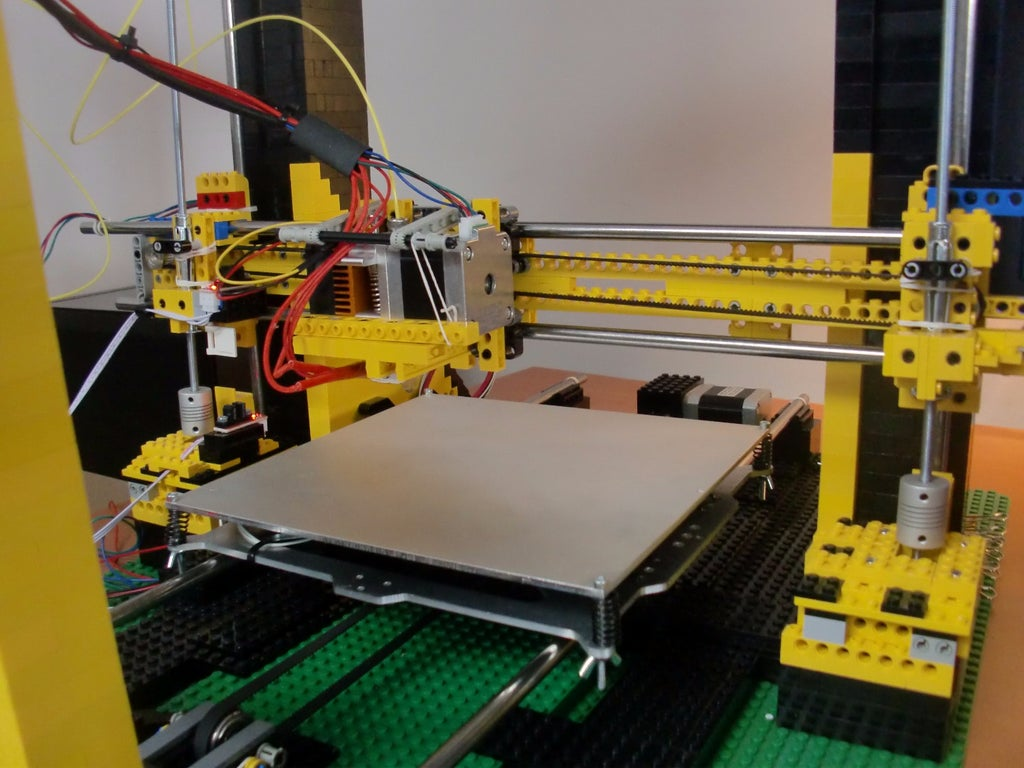
\includegraphics[height=5cm]{rapid-prototyping/lego-3d-printer.jpg}
        \caption{Lego \texttrademark: 3D Printer (Source: Instructables)}
    \end{figure}
\end{frame}
\subsection{Plaast/Instamorph}
\begin{frame}
    \begin{itemize}
        \item Heatable polymer
        \item Becomes soft with hot water
        \item Hard at room temperature
    \end{itemize}
    \begin{figure}
        % https://www.bengs-modellbau.de/material/baumaterial/plaast-kunststoff-1kg
        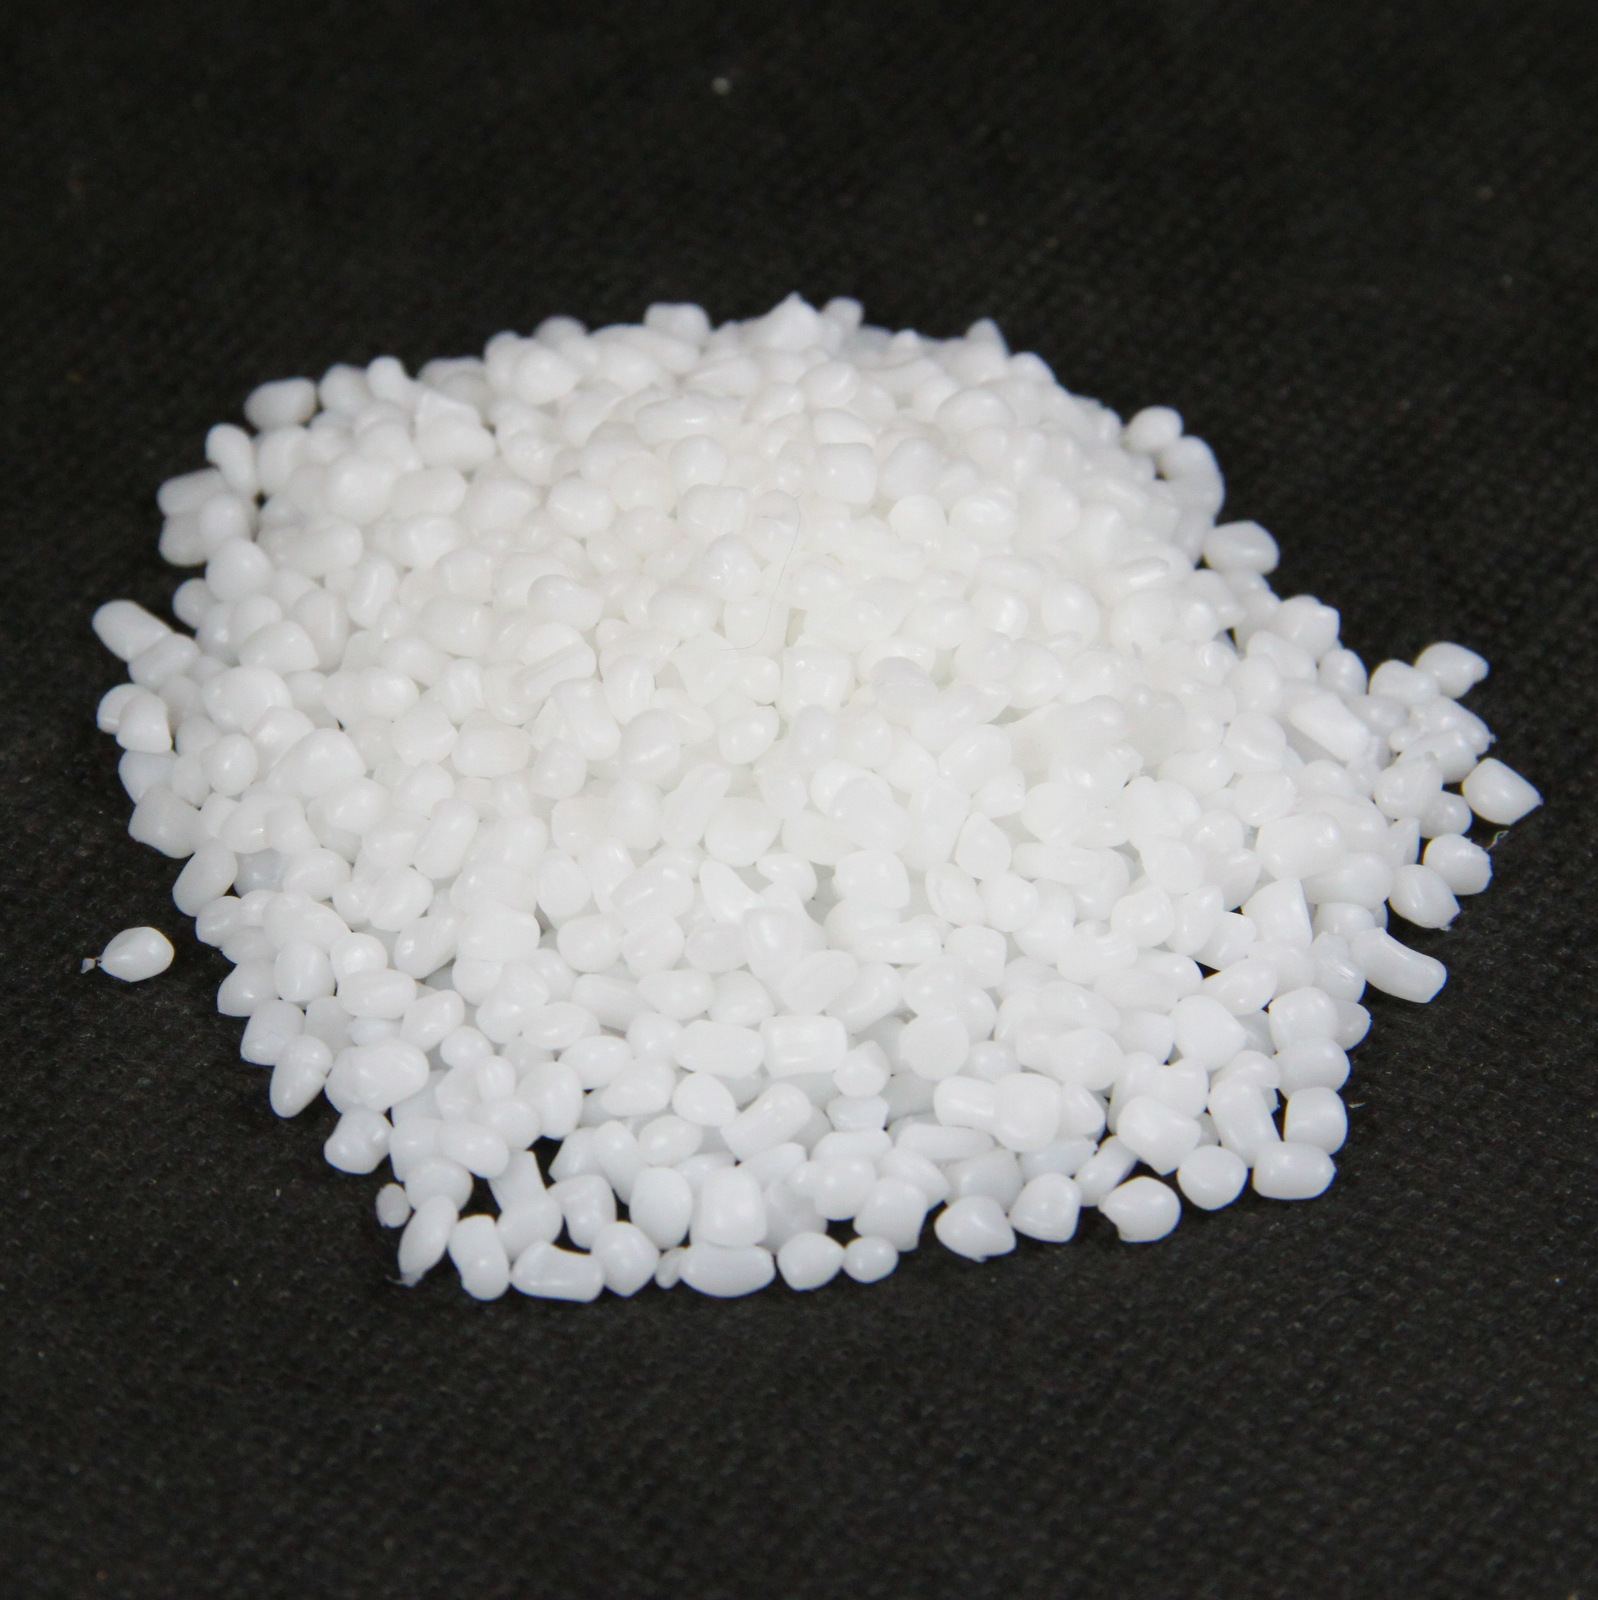
\includegraphics[height=5cm]{rapid-prototyping/plaast.jpg}
        \caption{Plaast (Polycaprolacton)}
    \end{figure}
\end{frame}

\begin{frame}
    \begin{figure}
        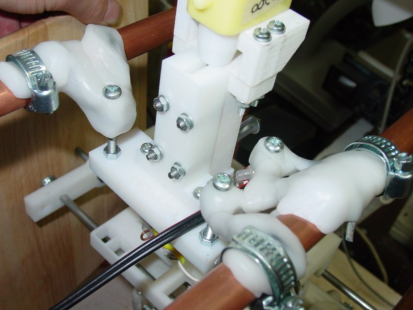
\includegraphics[height=6cm]{rapid-prototyping/plaast-pipes.pdf}
        \caption{Plaast: Pipes Mount}
    \end{figure}
\end{frame}

\subsection{\glsentrytext{pvc} Pipes}
\begin{frame}
    \begin{itemize}
        \item Very cheap
        \item Easy to obtain
        \item Does not require special tools/machines
        \item Therese Willkomm (``\acs{at} Solutions in Minutes'')
    \end{itemize}
    \begin{figure}
        % https://organizedclassroom.com/pvc-pipe-solutions/
        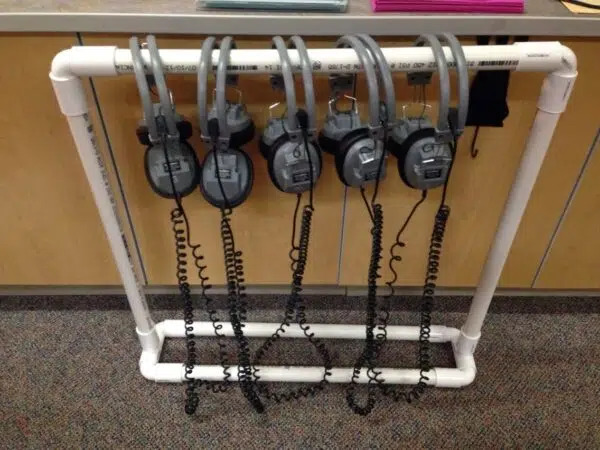
\includegraphics[height=4.5cm]{rapid-prototyping/pvc-pipes-headphone-stand.jpg}
        \caption{\glsentrytext{pvc} Pipes: Headphone Stand}
    \end{figure}
\end{frame}

\begin{frame}
    \begin{figure}
        % https://busybugs.co/2012/08/diy-sensory-water-table/
        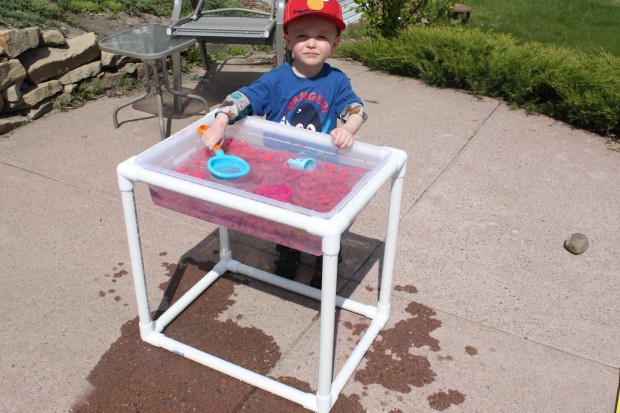
\includegraphics[width=\textwidth]{rapid-prototyping/pvc-pipes-sensory-table.jpg}
        \caption{\glsentrytext{pvc} Pipes: Sensory/Water Table}
    \end{figure}
\end{frame}

\begin{frame}
    \begin{figure}
        % https://www.pinterest.com/pin/331225747565285513/
        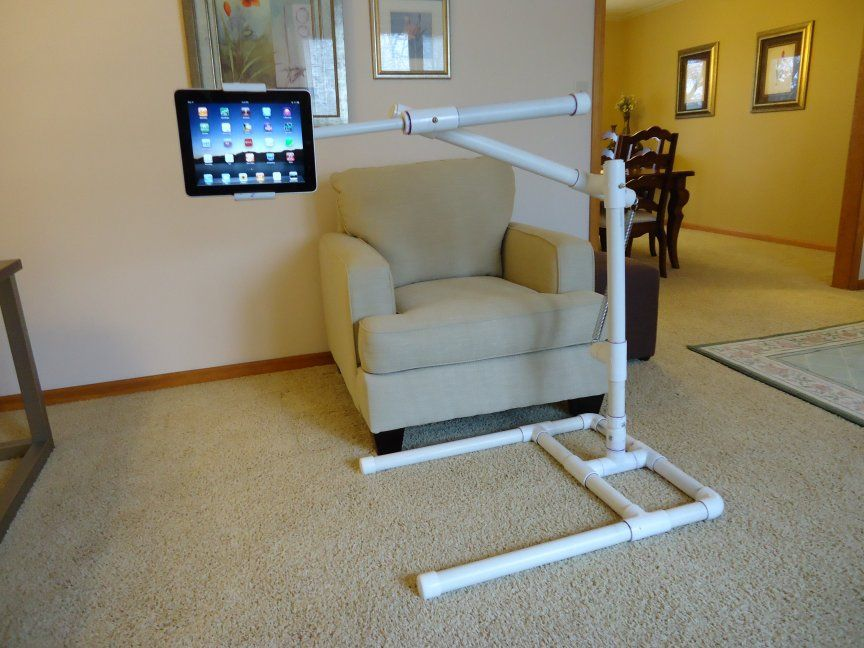
\includegraphics[height=7cm]{rapid-prototyping/pvc-pipes-ipad-holder.jpg}
        \caption{\glsentrytext{pvc} Pipes: iPad Holder}
    \end{figure}
\end{frame}
\subsection{LocLine}
\begin{frame}
    \begin{itemize}
        \item Cheap
        \item Easy to obtain
        \item Does not require special tools/machines
        \item From \acs{cnc} industry (coolant hose)
    \end{itemize}
    \begin{figure}
        % https://www.amazon.com/ModularHose-Compatible-Tablets-Samsung-Microsoft/dp/B087WTTMQR
        \includegraphics<1>[height=5cm]{rapid-prototyping/locline-tablet-holder-1.jpg}
        % https://www.pinterest.com/pin/497858933777199698/
        \includegraphics<2>[height=5cm]{rapid-prototyping/locline-tablet-holder-2.jpg}
        \caption{LocLine: Tablet Holder}
    \end{figure}
\end{frame}

\appendix

\begin{frame}[allowframebreaks]{Acronyms}
    \glsadd{pvc}
    \glsadd{sls}
    \printglossary[type=\acronymtype, nonumberlist]
\end{frame}

\begin{frame}[label=references]{References}
    \bibliography{references}
\end{frame}

\end{document}